Let's now analyze in some more detail some results presented in the previous section.

The mean \textbf{Source Buildability} of the projects (47.29\%), although low, is slightly higher than in previous studies on Java projects such as that of Tufano et al (38.13\%). 
This is partly due to having left out 20 projects whose compilability was 0.
But what is more interesting is the differences from project to project, something that was expected, and seen in previous studies on the matter~\cite{tufano2017there,sulir2020large,querel:2021:warning}.

The mean value of the \textbf{TestBuildability~\textsubscript{A}} is significantly lower (41.73\%), because SourceBuildability is a threshold for this metric.
Moreover, considering only those commits where the source code is compiled, the \textbf{TestBuildability~\textsubscript{S}} offers a considerably higher value on average (88\%).
This value is reasonable, since once the main source code was built, it is more likely that the test code can also be built. 
What is maybe unexpected, as we will discuss later in Section~\ref{sec:semantics}, is that it is not even higher.
We also note that for this metric, 50\% of the projects offer a value higher than 97\%.


%In contrast, it seems that the buildability of both source code and tests is significantly lower than for projects collected through the GitHub API. Many4J projects offer a significantly lower mean on all parameters.

The most clear result when analyzing testability of projects is its variability from project to project. 
Figure~\ref{fig:testability-overview} illustrates this, by showing the shape of the distribution of all testability metrics we defined, for all projects.

\begin{figure*}[ht!]
    \centering    
    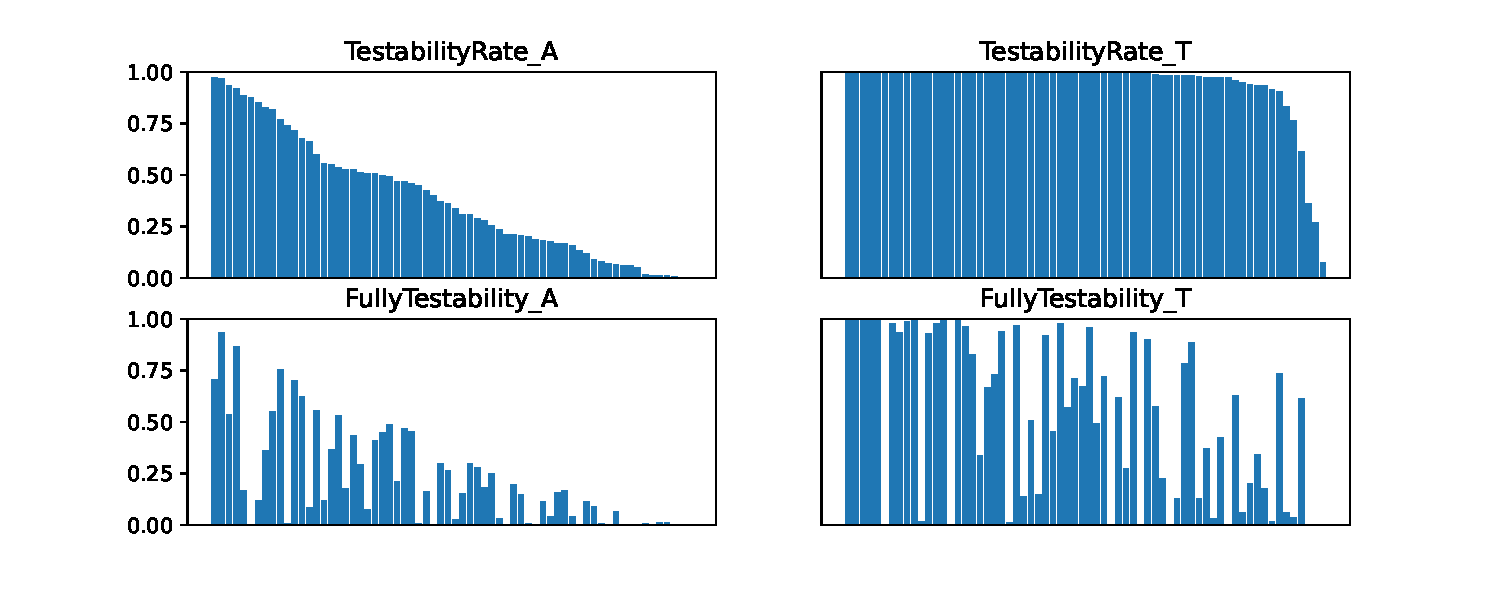
\includegraphics[width=16cm]{pages/02-Testability/images/Overview.pdf}
    \vspace{-0.5cm}
    \caption{Overview of testabilities - Each bar represents a project. Each column is ordered by the corresponding TestabilityRate (A and T) of each project.}
    \label{fig:testability-overview}
\end{figure*}

Looking at the Testability Rate values, when we focus on those commits where the tests can be built (\textbf{TestabilityRate\textsubscript{T}}) we observe an average value of 94.14\%, a high percentage of the project's tests are executed successfully. 
% Again, we see that the \textbf{TestabilityRate\textsubscript{T}}, as with other values, varies a lot between projects, with the median of this value being 99.53\%, indicating that in 50\% of the cases almost all the tests pass for test buildable commits.
By calculating the TestabilityRate considering all commits (\textbf{TestabilityRate\textsubscript{A}}), this value gives an overview of the testability of the project and how Source Buildability impacts running tests on past commits.

Focusing on \textbf{FullyTestability\textsubscript{T}}, we could expect it would be usually high: developers should write code that does not break \textit{all} the tests. 
Fact is that in more than half of the commits that were test-buildable some tests fail when they are run. 
This result, which may seem surprising, deserves as well more discussion that we will provide in Section~\ref{sec:low-testability}.

\textbf{FullyTestability\textsubscript{A}} gives quite interesting information: the fraction of commits that are testable, with respect to the total number of commits. 
When buildability is low, this fraction is necessarily low, just meaning that commits are not testable because they are not source- or test-buildable. 
When buildability is high, \textit{FullyTestability\textsubscript{A}} really shows differences. 

With the data presented up to here, we can already answer RQ\textsubscript{1}, RQ\textsubscript{2} and RQ\textsubscript{3}:

\vspace{0.5cm}
\fbox{\begin{minipage}{\textwidth}
\textbf{\textbf{RQ\textsubscript{1}}: ``\RQI''}
We found 93,925 test-buildable commits out of 103,097 source-buildable commits.
When calculating \textit{TestBuildability} using all the commits of the project we obtain an average value of 41.73\%, while if we compute only the commits in which we can build the source code, the average value increases significantly (88.2\%).
\end{minipage}}

\vspace{0.5cm}
\fbox{\begin{minipage}{\textwidth}
\textbf{\textbf{RQ\textsubscript{2}}: ``\RQII''}
We found 40,540 fully-testable commits out of 93,925 test-buildable commits. 
When calculating \textit{FullyTestability} using all the commits of the project we obtain an average value of 22.12\%, while if we compute only the commits in which we can build the tests, the average value increases significantly (52.53\%).
\end{minipage}}

\vspace{0.5cm}
\fbox{\begin{minipage}{\textwidth}
\textbf{\textbf{RQ\textsubscript{3}}: ``\RQIII''}
When calculating \textit{TestabilityRate} using all the commits of the project we obtain an average value of 38.63\%, while if we compute only the commits in which we can build the tests, the average value increases significantly (94.14\%).
\end{minipage}}
    
